\documentclass{ctexart}
\usepackage{PhysicalChemistryNote}

\begin{document}\pagestyle{plain}
\noindent\tbf{\LARGE 4D 多组分系统的相变与相图}\vspace{15pt}\\
\indent 在经历了漫长的对溶液的讨论后,我们终于来到了多组分系统与相图这一节.%
尽管我们没有对多组分系统相变的规律进行总结,不过我们在\tbf{4C}已经不计其数地使用了多组分系统相平衡的条件.%
因此,本节事实上没有多少新的知识,更多的是总结与归纳,以及引入一些新的方法描述多组分系统各相的平衡情况.\vspace{12pt}\\
\Section{4D.1 多组分系统的相律}
\indent 我们已经在\tbf{4A.1.7}中不加证明地给出了单组分系统的相律.对于更一般的多组分系统,%
我们也需要给定一定数量的状态函数(例如温度$T$,压力$p$等等)来确定系统的状态.%
可以想见,需要给定的条件数应当与系统中的组分数和相数都有关系.下面我们来确定其具体关系式.
\begin{derivation}
    考虑某个平衡的系统,组分数为$S$,相数为$\varPhi$,并且假定各组分在每个相中都存在,且不发生化学反应.\\
    采取摩尔分数$x_i$表示每个相的组成.因为有$\displaystyle\sum_{i=1}^{k}x_i=1$的限制存在,%
    于是每个相都需要$S-1$个独立的变量以描述其组成.由于相数为$\varPhi$,再加上相平衡时各相的温度$T$和压力$p$,%
    就需要$\varPhi(S-1)+2$个变量描述该系统.\\
    然而,由于我们需要保证各组分在各相中的化学势$\mu$相等,于是就有
    \[\mu_{i,\alpha}=\mu_{i,\beta}=\cdots=\mu_{i,\phi}(i=1,2,\cdots,S)\]
    其中$\alpha,\beta,\cdots,\phi$为系统的所有$\varPhi$个相.\\
    由于化学势是温度$T$,压力$p$和摩尔分数$x_i$的函数,因此对于每个$i$,只需任意地确定某一相$\lambda$中的$x_{i,\lambda}$,%
    就可以通过上述等量关系求得所有相中的$x_i$.因此,对于每个组分$i$,上述等式意味着$\varPhi-1$个需要满足的等量关系,一共就有$S(\varPhi-1)$个需要满足的等量关系.\\
    每个等量关系都可以使我们描述系统的独立变量减少$1$个.根据自由度的定义,就有
    \[f=\left(\varPhi(S-1)+2\right)-\left(S(\varPhi-1)\right)=S-\varPhi+2\]
    稍作整理,就可得
    \[\varPhi+f=S+2\]
    推广而言,如果某一组分$i$在某一相$\lambda$中不存在,那么$x_{i,\lambda}$就不需要被描述,保证化学势相等的等量关系也减少一个.%
    这样,变量数和等量关系同步减少,对我们的结论没有影响.
\end{derivation}
\begin{theorem}[4D.1.1 简单多组分系统的相律]
    对于一个不发生化学反应的系统,其自由度$f$满足
    \[\varPhi+f=S+2\]
    其中$S$为系统的组分数,$\varPhi$为系统的相数.
\end{theorem}
对于可能发生化学反应的系统,根据我们在普通化学中学过的知识可知一个平衡相当于一个等量关系,%
相当于这些组分之间并不独立.为此,我们需要把组分数$S$改写成独立组分数$C$,即总的组分数减去需要满足的平衡关系数.\\
\indent 对于凝聚态系统(例如具有很低的蒸气压的液体和固体),压力对系统的改变可以忽略,此时等式右边的$2$也可以改写为$1$.\\
\indent 总结上述讨论,我们可以得出相律的更一般的形式,它由Gibbs在1877年首次提出.
\begin{theorem}[4D.1.2 Gibbs相律]
    多组分系统的自由度$f$满足
    \[\varPhi+f=C+n\]
    其中$C$为系统的\tbf{独立组分数},$\varPhi$为系统的相数,$n$为外界因素的数目(多数时候取$2$,代表温度$T$和压力$p$;%
    如果压力对系统影响可忽略不计,那么也可以取$n=1$).
\end{theorem}
Gibbs相律是我们描述多组分系统的相图时所应当遵守的基本规律.\\
\indent 对于双组分系统,$S=2$,就有$f=4-\varPhi$.由于我们讨论的系统至少有一个相,%
因此,系统的状态可以用至多三个变量来确定.我们一般采取温度$T$,压力$p$和组成$x$描述其状态,%
这样系统的相图就是一个具有三个坐标轴的立体图.\\
\indent 实际情况中,我们常常采取固定某一变量的方法描述双组分系统的相图(即上述立体图的截面).%
通常来说,我们会使用$p-x$图和$T-x$图描述系统的状态.我们将在接下来的几节中介绍各种双组分系统的相图.\vspace{12pt}\\
\Section{4D.2 双组分溶液的相图}
\Part{双组分理想溶液的相图}
\indent 我们先讨论$p-x$图.
\begin{derivation}
    根据Raoult定律,组分$A$和组分$B$形成的理想溶液满足
    \[\left\{\begin{array}{l}
        p_A=p_A^\ast x_{A,\l}\\
        p_B=p_B^\ast\left(1-x_{A,\l}\right)
    \end{array}\right.\]
    于是总蒸气压
    \[p=p_A+p_B=p_B^\ast+\left(p_A^\ast-p_B^\ast\right)x_{A,\l}\]
    如果我们以$x_{A,\l}$为横轴,$p$为纵轴,就可以得到如下的相图.
    \begin{center}
        \documentclass{standalone}
\usepackage{PhysicalChemistryNote}
\begin{document}
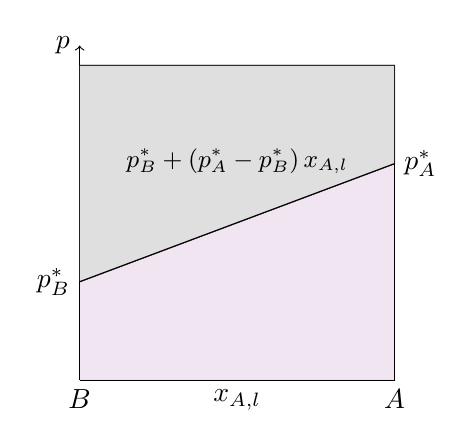
\begin{tikzpicture}
    \draw[-] (0,0) -- (4,0);
    \draw[->] (0,0) -- (0,4.25) node[left]{$p$};
    \draw[-] (4,0) -- (4,4);
    \draw[-] (0,4) -- (4,4);
    \node[below] at (0,0) {$B$};
    \node[below] at (4,0) {$A$};
    \node[below] at (2,0) {$x_{A,\l}$};
    \filldraw[fill=lightgray,opacity=0.5] (0,1.25) -- (4,2.75) -- (4,4) -- (0,4);
    \filldraw[fill=violet,opacity=0.1] (0,1.25) -- (4,2.75) -- (4,0) -- (0,0);
    \node[left] at (0,1.25) {$p_B^\ast$};
    \node[right] at (4,2.75) {$p_A^\ast$};
    \node[above] at (2,2.5) {\small{$p_B^\ast+\left(p_A^\ast-p_B^\ast\right)x_{A,\l}$}};
    \draw[-] (0,1.25) -- (4,2.75);
    
\end{tikzpicture}
\end{document}
    \end{center}
    其中上面灰色的部分为液相,下面紫色的部分为气相.可以看到,选取某组分在液相中的摩尔分数$x_\l$和压力$p$,%
    作出的理想溶液相图中两相的分界线为直线.\\
    显而易见的,两种组分在气相中的含量与它们在液相中的含量并不相同.我们有
    \[x_{A,\g}=\dfrac{p_A}{p}=\dfrac{p_A^\ast x_{A,\l}}{p_B^\ast+\left(p_A^\ast-p_B^\ast\right)x_{A,\l}}\]
    于是
    \[x_{A,\l}=\dfrac{p_B^\ast x_{A,\g}}{p_A^\ast+\left(p_B^\ast-p_A^\ast\right)x_{A,\g}}\]
    从而
    \[p=p_B^\ast+\dfrac{p_B^\ast x_{A,\g}\left(p_A^\ast-p_B^\ast\right)}{p_A^\ast+\left(p_B^\ast-p_A^\ast\right)x_{A,\g}}
    =\dfrac{p_A^\ast p_B^\ast}{p_A^\ast+\left(p_B^\ast-p_A^\ast\right)x_{A,\g}}\]
    我们以$x_{A,\g}$为横轴,$p$为纵轴,可以得到如下的相图.
    \begin{center}
        \documentclass{standalone}
\usepackage{PhysicalChemistryNote}
\begin{document}
\begin{tikzpicture}
    \draw[-] (0,0) -- (4,0);
    \draw[->] (0,0) -- (0,4.25) node[left]{$p$};
    \draw[-] (4,0) -- (4,4);
    \draw[-] (0,4) -- (4,4);
    \node[below] at (0,0) {$B$};
    \node[below] at (4,0) {$A$};
    \node[below] at (2,0) {$x_{A,\g}$};
    \draw[domain=0:4] plot[smooth](\x,{4*1.25*2.75/(11-1.5*\x)});
    \filldraw[fill=lightgray,opacity=0.5,domain=0:4] plot[smooth](\x,{4*1.25*2.75/(11-1.5*\x)}) -- (4,4) -- (0,4);
    \filldraw[fill=violet,opacity=0.1,domain=0:4] plot[smooth](\x,{4*1.25*2.75/(11-1.5*\x)}) -- (4,0) -- (0,0);
    \node[left] at (0,1.25) {$p_B^\ast$};
    \node[right] at (4,2.75) {$p_A^\ast$};
    \node[below] at (2,1.5) {\small{$\dfrac{p_A^\ast p_B^\ast}{p_A^\ast+\left(p_B^\ast-p_A^\ast\right)x_{A,\g}}$}};
    
    
\end{tikzpicture}
\end{document}
    \end{center}
    可以看到,以气相中$A$的摩尔分数作出的相图的分界线是一条下凹的曲线,总是处于液相线之下.如果我们把两条线画在同一张图中,就有
    \begin{center}
        \documentclass{standalone}
\usepackage{PhysicalChemistryNote}
\begin{document}
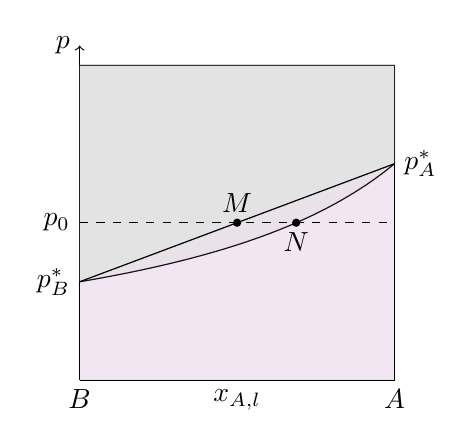
\begin{tikzpicture}
    \draw[-] (0,0) -- (4,0);
    \draw[->] (0,0) -- (0,4.25) node[left]{$p$};
    \draw[-] (4,0) -- (4,4);
    \draw[-] (0,4) -- (4,4);
    \node[below] at (0,0) {$B$};
    \node[below] at (4,0) {$A$};
    \node[below] at (2,0) {$x_{A,\l}$};
    \draw[domain=0:4] plot[smooth](\x,{4*1.25*2.75/(11-1.5*\x)});
    \filldraw[fill=lightgray,opacity=0.25,domain=0:4] plot[smooth](\x,{4*1.25*2.75/(11-1.5*\x)}) -- (4,4) -- (0,4);
    \filldraw[fill=violet,opacity=0.05,domain=0:4] plot[smooth](\x,{4*1.25*2.75/(11-1.5*\x)}) -- (4,0) -- (0,0);
    \filldraw[fill=lightgray,opacity=0.25] (0,1.25) -- (4,2.75) -- (4,4) -- (0,4);
    \filldraw[fill=violet,opacity=0.05] (0,1.25) -- (4,2.75) -- (4,0) -- (0,0);
    \node[left] at (0,1.25) {$p_B^\ast$};
    \node[left] at (0,2) {$p_0$};
    \node[right] at (4,2.75) {$p_A^\ast$};
    \draw[-] (0,1.25) -- (4,2.75);
    \draw[dashed] (0,2) -- (4,2);
    \fill (2,2) circle (1.5pt) node[above]{$M$};
    \fill (2.75,2) circle (1.5pt) node[below]{$N$};
    
\end{tikzpicture}
\end{document}
    \end{center}
    根据相律,在两相平衡时系统的自由度为$f=C+n-\varPhi=2+2-0$,只要给定压强$p_0$和温度$T$就可以确定其组成和状态.因此,%
    我们作一条直线$p=p_0$分别交两条分界线于$M,N$两点,就可以知道此时两相平衡时液相和气相的组成.\\
    容易看出在平衡时,蒸气压大的组分在气相中的摩尔分数总是比在液相中的摩尔分数高.
\end{derivation}
通常来说,我们更常在恒定压力下对系统进行改变,例如蒸馏和精馏等操作.%
因此,$T-x$图更为常用.
\begin{derivation}\setcounter{equation}{0}
    我们仍然讨论由组分$A$和组分$B$组成的理想溶液,并保持总压力为$p$不变.\\
    根据Clausius-Clapeyron方程有
    \begin{equation}
        \dfrac{\di\ln p_{i}^\ast}{\di T}=\dfrac{\Delta_\vap H_{\m,i}}{RT^2}
    \end{equation}
    其中$i=A,B$.我们再假定摩尔蒸发焓随温度变化很小,设纯的$i$在$p$下的沸点为$T_i^\ast$,对(1)定积分有
    \begin{equation}
        \ln\dfrac{p_i^\ast}{p}=\dfrac{\Delta_\vap H_{\m,i}}{R}\left(\dfrac{1}{T_i^\ast}-\dfrac1T\right)
    \end{equation}
    移项并取指数就有
    \begin{equation}
        p_i^\ast=p\exp{\left[\dfrac{\Delta_\vap H_{\m,i}}{R}\left(\dfrac{1}{T_i^\ast}-\dfrac1T\right)\right]}
    \end{equation}
    根据Raoult定律有
    \begin{equation}
        p=p_{A}^\ast x_{A,\l}+p_B^\ast\left(1-x_{A,\l}\right)
    \end{equation}
    将(3)代入其中就有
    \begin{equation}
        x_{A,\l}\exp{\left[\dfrac{\Delta_\vap H_{\m,A}}{R}\left(\dfrac{1}{T_A^\ast}-\dfrac1T\right)\right]}
        +\left(1-x_{A,\l}\right)\exp{\left[\dfrac{\Delta_\vap H_{\m,B}}{R}\left(\dfrac{1}{T_B^\ast}-\dfrac1T\right)\right]}=1
    \end{equation}
    这就给出了$T$与$x_{A,\l}$的函数关系,绘制出的相图如下所示.
    \begin{center}
        \documentclass{standalone}
\usepackage{PhysicalChemistryNote}
\begin{document}
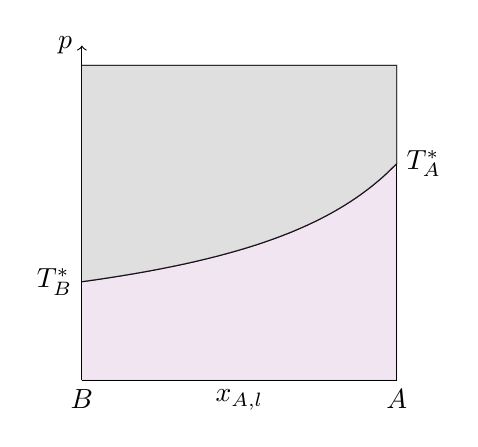
\begin{tikzpicture}
    \draw[-] (0,0) -- (4,0);
    \draw[->] (0,0) -- (0,4.25) node[left]{$p$};
    \draw[-] (4,0) -- (4,4);
    \draw[-] (0,4) -- (4,4);
    \node[below] at (0,0) {$B$};
    \node[below] at (4,0) {$A$};
    \node[below] at (2,0) {$x_{A,\l}$};
    \draw[domain=0:4] plot[smooth](\x,{1/ln(0.1967*(11.3117-\x))});
    \filldraw[fill=lightgray,opacity=0.5,domain=0:4] plot[smooth](\x,{1/ln(0.1967*(11.3117-\x))}) -- (4,4) -- (0,4);
    \filldraw[fill=violet,opacity=0.1,domain=0:4] plot[smooth](\x,{1/ln(0.1967*(11.3117-\x))}) -- (4,0) -- (0,0);
    \node[left] at (0,1.25) {$T_B^\ast$};
    \node[right] at (4,2.75) {$T_A^\ast$}; 
    
\end{tikzpicture}
\end{document}
    \end{center}
    如果将$p_A+p_B=p$和$x_{A,\g}$代入(3)可得
    \begin{equation}
        x_{A,\g}\exp{\left[\dfrac{\Delta_\vap H_{\m,A}}{R}\left(\dfrac{1}{T_A^\ast}-\dfrac1T\right)\right]}
        =\left(1-x_{A.,\g}\right)\exp{\left[\dfrac{\Delta_\vap H_{\m,B}}{R}\left(\dfrac{1}{T_B^\ast}-\dfrac1T\right)\right]}
    \end{equation}
\end{derivation}

\end{document}